% !TEX program = xelatex
\documentclass[12pt,a4paper]{article}
\usepackage[left=3cm,right=2cm,top=2.5cm,bottom=2.5cm]{geometry}
\usepackage{fontspec}
\setmainfont{Times.TTF}[Path=fonts/,BoldFont=Timesbd.TTF,ItalicFont=Timesi.TTF,BoldItalicFont=Timesbi.TTF]
\usepackage[vietnamese]{babel}
\usepackage{amsmath,amssymb,booktabs,tabularx,array,graphicx}
\usepackage[table]{xcolor}
\usepackage{titlesec,enumitem,caption,float,fancyhdr}
\usepackage{hyperref}
\definecolor{accent}{HTML}{216477}
\definecolor{pale}{HTML}{EAF3F5}
\definecolor{ink}{HTML}{243746}
\hypersetup{colorlinks=true,linkcolor=ink,citecolor=accent,urlcolor=accent,
 pdftitle={Đánh giá và cải tiến truy xuất bằng chứng pháp lý cho hỏi đáp pháp luật Việt Nam},
 pdfauthor={Lê Minh Nhựt; Phan Văn Thắng; Phan Tiến}}
\urlstyle{same}
\linespread{1.15}
\setlength{\parindent}{0.65cm}
\setlength{\parskip}{3pt}
\setlength{\emergencystretch}{2em}
\titleformat{\section}{\large\bfseries\color{ink}}{\thesection}{0.65em}{}
\titleformat{\subsection}{\normalsize\bfseries}{\thesubsection}{0.65em}{}
\titlespacing*{\section}{0pt}{12pt}{7pt}
\titlespacing*{\subsection}{0pt}{9pt}{4pt}
\setlist[itemize]{leftmargin=1.5em,itemsep=3pt,topsep=3pt}
\captionsetup{font=small,labelfont=bf,labelsep=period,skip=6pt}
\renewcommand{\tablename}{Bảng}
\renewcommand{\figurename}{Hình}
\renewcommand{\contentsname}{Mục lục}
\addto\captionsvietnamese{\renewcommand{\refname}{Tài liệu tham khảo}\renewcommand{\contentsname}{Mục lục}}
\setcounter{tocdepth}{1}
\pagestyle{fancy}
\fancyhf{}
\fancyhead[L]{\small\color{gray}Truy xuất bằng chứng pháp lý trên VLSP 2025 DRiLL}
\fancyfoot[C]{\thepage}
\renewcommand{\headrulewidth}{0.3pt}
\setlength{\headheight}{16pt}
\newcolumntype{Y}{>{\raggedright\arraybackslash}X}
\newcommand{\best}[1]{\textbf{#1}}
\newcommand{\id}[1]{\texttt{#1}}
\begin{document}
% 1 — Bìa.
\thispagestyle{empty}
\begin{center}
{\large ĐẠI HỌC QUỐC GIA THÀNH PHỐ HỒ CHÍ MINH}\\[5pt]
{\large\bfseries TRƯỜNG ĐẠI HỌC CÔNG NGHỆ THÔNG TIN}\\[5pt]
{\normalsize KHOA KHOA HỌC VÀ KỸ THUẬT THÔNG TIN}
\vspace{1.8cm}

{\Large\bfseries BÁO CÁO ĐỒ ÁN}\\[10pt]
{\large HỌC MÁY TIÊN TIẾN VÀ ỨNG DỤNG}
\vspace{1.4cm}

{\LARGE\bfseries\color{ink} ĐÁNH GIÁ VÀ CẢI TIẾN\\[7pt]
TRUY XUẤT BẰNG CHỨNG PHÁP LÝ\\[7pt]
CHO HỎI ĐÁP PHÁP LUẬT VIỆT NAM}\\[16pt]
{\large Nghiên cứu trên VLSP 2025 DRiLL}
\vspace{1.3cm}

\rule{0.72\textwidth}{0.6pt}\\[16pt]
{\large\textbf{Giảng viên hướng dẫn:} TS. Hà Minh Tân}\\[18pt]
{\large\textbf{Nhóm thực hiện:} Nhóm 18}\\[12pt]
\begin{tabular}{lr}
Lê Minh Nhựt & 26848158\\[6pt]
Phan Văn Thắng & 26848203\\[6pt]
Phan Tiến & 26848224
\end{tabular}
\vfill
Thành phố Hồ Chí Minh, tháng 11 năm 2026
\end{center}
% 2 — Tóm tắt và mục lục.
\clearpage
\section*{Tóm tắt}
\noindent Truy xuất bằng chứng là thành phần quan trọng của hệ thống hỏi đáp pháp luật: một câu hỏi có thể cần nhiều điều luật để xác định đối tượng, điều kiện và ngoại lệ. Báo cáo nghiên cứu ảnh hưởng của biểu diễn văn bản, kết hợp nguồn truy xuất, xếp hạng lại và lựa chọn số bằng chứng trên VLSP 2025 DRiLL. Kho dữ liệu gồm 59\,628 điều luật có nội dung; 2\,190 câu hỏi có nhãn được chia thành 1\,752 câu huấn luyện và 438 câu phát triển. Hệ thống sử dụng Article window 448 token, chồng lấn 64 token; kết hợp BM25, VietLegal-Harrier và multilingual-E5-large bằng Weighted Reciprocal Rank Fusion (WRRF). Vietnamese Reranker được tinh chỉnh theo nhãn cấp Điều để chấm 50 đoạn ứng viên, sau đó lấy điểm lớn nhất theo mã điều luật. LightGBM tổng hợp 57 đặc trưng để xếp hạng và Multiclass--Ridge chọn số điều luật phù hợp với từng câu hỏi. Trên tập phát triển, truy xuất lai đạt Macro-$F_2$ 0.5252 tại top-2; các mốc sau xếp hạng lại, tổng hợp tín hiệu và chọn số điều luật lần lượt là 0.5967, 0.6217 và 0.6910. Kết quả đánh giá cuối cùng đạt Macro-$F_2$ 0.6978 trên public và 0.6825 trên private. Kết quả cho thấy việc đưa bằng chứng lên đầu và điều chỉnh độ dài đầu ra bổ sung cho khả năng tìm ứng viên của truy xuất lai. Các thành phần hỏi đáp sau quy trình truy xuất chỉ phục vụ minh họa ứng dụng, nằm ngoài trọng tâm nghiên cứu của nhóm.

\noindent\textbf{Mã nguồn:} \url{https://github.com/leeminsun1205/Drill-reliable-retrieval}.

\noindent\textbf{Từ khóa:} truy xuất pháp luật; DRiLL; truy xuất lai; xếp hạng lại; LightGBM; chọn số bằng chứng.
\vspace{4pt}
\begingroup\small\tableofcontents\endgroup
% 3 — Giới thiệu.
\clearpage
\section{Giới thiệu}\label{sec:intro}
\subsection{Bối cảnh và phát biểu bài toán}
Trong hỏi đáp pháp luật, một câu trả lời có thể cần đồng thời quy định về đối tượng, điều kiện áp dụng và ngoại lệ. Vì vậy, chỉ tìm văn bản cùng chủ đề chưa đủ: hệ thống phải trả về đúng các điều luật liên quan và hạn chế bỏ sót bằng chứng. Trong kiến trúc tăng cường truy xuất cho tạo sinh (Retrieval-Augmented Generation, RAG)~\cite{rag}, truy xuất cung cấp ngữ cảnh cho mô hình ngôn ngữ. Truy xuất đúng bằng chứng giúp mô hình tạo câu trả lời có căn cứ. Mô hình vẫn cần hiểu đúng nội dung và điều kiện áp dụng của các điều luật để diễn giải chính xác.

Đồ án tập trung vào \textbf{truy xuất và lựa chọn bằng chứng cấp Điều} trên VLSP 2025 DRiLL~\cite{drill}. Cho câu hỏi tiếng Việt $q$ và kho điều luật $\mathcal{D}$, hệ thống tạo danh sách có thứ hạng
\begin{equation}
\widehat{A}_q=(a_1,a_2,\ldots,a_{k_q}),\qquad a_i\in\mathcal{D},\quad a_i\ne a_j\ (i\ne j).
\label{eq:task}
\end{equation}
Mỗi $a_i$ được nhận diện bằng mã \id{aid}; $k_q$ là số điều luật được trả về cho câu hỏi. Nhãn $G_q$ là tập \id{aid} liên quan do dữ liệu gán nhãn cung cấp (tập gold). Mục tiêu là trả về đúng và đủ các điều luật trong $G_q$. Các đoạn văn bản (chunk) là đơn vị xử lý trung gian; kết quả cuối cùng vẫn được đối chiếu theo mã điều luật.

Ví dụ, câu hỏi mã 730 trong dữ liệu là \emph{``Viên chức có được tạm hoãn nghĩa vụ quân sự không?''}; tập gold gồm hai mã điều luật 55075 và 4993, lần lượt thuộc văn bản 78/2015/QH13 và 48/2019/QH14. Ví dụ cho thấy đơn vị đầu ra cần là tập điều luật liên quan, có thể thuộc nhiều văn bản.
\subsection{Câu hỏi nghiên cứu và đóng góp}
Bốn câu hỏi xuyên suốt báo cáo là: (1) biểu diễn điều luật thế nào để truy xuất hiệu quả; (2) kết hợp từ vựng, ngữ nghĩa và xếp hạng lại đóng góp ra sao; (3) LightGBM có cải thiện thứ hạng khi tổng hợp nhiều tín hiệu; (4) chọn số điều luật theo từng câu hỏi có tốt hơn top-$k$ cố định không? Các đóng góp thực nghiệm gồm:
\begin{itemize}
\item So sánh biểu diễn điều luật và các thành phần truy xuất trên cùng phân hoạch, từ đó chọn Article window và truy xuất lai ba nguồn.
\item Xây dựng chuỗi chấm điểm đoạn, gộp về điều luật và tổng hợp tín hiệu; so sánh các nhóm đặc trưng LightGBM với giao thức ngoài mẫu theo câu hỏi.
\item Đánh giá cách chọn số điều luật từ danh sách đã xếp hạng, phân tích lỗi theo từng bước và đối chiếu bản nộp với các hệ thống trên DRiLL.
\end{itemize}
Phần~\ref{sec:related} đặt các lựa chọn trong nghiên cứu liên quan; Phần~\ref{sec:method} mô tả phương pháp; Phần~\ref{sec:experiments} phân tích thực nghiệm; Phần~\ref{sec:conclusion} tổng kết ứng dụng và giới hạn.
% 4 — Liên quan.
\clearpage
\section{Cơ sở và nghiên cứu liên quan}\label{sec:related}
\textbf{Truy xuất từ vựng và ngữ nghĩa.} BM25~\cite{bm25} chấm mức khớp từ, có xét độ hiếm của từ và độ dài văn bản; phù hợp với thuật ngữ hoặc số hiệu xuất hiện chính xác. Bi-encoder mã hóa câu hỏi và đoạn độc lập để tìm kiếm bằng vector. multilingual-E5-large (E5)~\cite{e5} cung cấp biểu diễn ngữ nghĩa dùng chung cho nhiều ngôn ngữ; VietLegal-Harrier (Harrier)~\cite{harrier} là mô hình hướng tới miền pháp luật tiếng Việt. Hai kiểu tín hiệu bổ sung nhau nhưng điểm thô khác thang, dẫn tới nhu cầu hợp nhất thứ hạng bằng RRF~\cite{rrf}.

\textbf{Xếp hạng lại và tổng hợp tín hiệu.} Cross-encoder đọc đồng thời câu hỏi và văn bản nên có thể xét tương tác chi tiết hơn bi-encoder~\cite{rerankbert}. Đổi lại, mỗi ứng viên cần một lượt chấm cặp, do đó chỉ áp dụng sau bước truy xuất. Vietnamese Reranker~\cite{vnreranker} cung cấp điểm khởi đầu phù hợp tiếng Việt. Sau đó, LightGBM~\cite{lightgbm} học quan hệ phi tuyến giữa điểm mô hình, thứ hạng, độ đồng thuận và đặc điểm đoạn. Trong đồ án, LightGBM ước lượng mức liên quan của từng cặp câu hỏi--điều luật để xếp lại danh sách ứng viên.

Bảng~\ref{tab:related} tóm tắt các hệ thống cùng bài toán. Các kết quả private là số công bố trên cùng benchmark, cung cấp mốc đối chiếu cho đồ án.
\begin{table}[H]
\centering\small
\caption{Nghiên cứu tiêu biểu trên VLSP 2025 DRiLL.}\label{tab:related}
\renewcommand{\arraystretch}{1.18}
\begin{tabularx}{\textwidth}{@{}>{\raggedright\arraybackslash}p{2.5cm}Y>{\raggedright\arraybackslash}p{1.3cm}Y@{}}
\toprule Hệ thống & Cách tiếp cận chính & $F_2$ private & Đặc điểm đối chiếu\\\midrule
Ban tổ chức~\cite{drill} & BM25 và cross-encoder hai giai đoạn & 0.5512 & Truy xuất hai giai đoạn, trả về top-2 cố định.\\
FPT IS~\cite{fpt} & Tăng cường dữ liệu, chia đoạn phân cấp, sử dụng LLM & 0.6966 & Bổ sung dữ liệu và bước xử lý bằng LLM.\\
EDM~\cite{edm} & Truy xuất nhiều giai đoạn, học xếp hạng và tín hiệu LLM & 0.7261 & Kết hợp nhiều tầng xếp hạng và chọn ngưỡng đầu ra.\\\bottomrule
\end{tabularx}
\end{table}
Bảng~\ref{tab:related} cho thấy các hệ thống cùng kết hợp truy xuất và xếp hạng lại, nhưng khác cách bổ sung tín hiệu và chọn kết quả. Ở bước chọn đầu ra, EDM~\cite{edm} lọc các ứng viên bằng ngưỡng điểm LightGBM được chọn trên tập phát triển. Đồ án nghiên cứu cách học độ dài danh sách cho từng câu hỏi bằng learned stopping và Multiclass--Ridge. Điểm khác biệt nằm ở việc dùng phân bố và khoảng cách điểm để quyết định giữ bao nhiêu điều luật. Cách này thích ứng với câu hỏi cần một hoặc nhiều bằng chứng, đồng thời tận dụng các điểm xếp hạng đã có. Hiệu quả được đánh giá qua so sánh với top-2 cố định và score gap ở Phần~\ref{sec:experiments}.
% 5 — Tổng thể.
\clearpage
\section{Phương pháp}\label{sec:method}
\subsection{Quy trình và đơn vị xử lý}
Hình~\ref{fig:pipeline} trình bày quy trình từ kho văn bản và câu hỏi đến các điều luật được chọn. Phần chuẩn bị được thực hiện trước: kho văn bản được tổ chức theo điều luật để lập chỉ mục BM25; mỗi điều luật đồng thời được chia thành các đoạn và mã hóa bằng Harrier, E5 để tạo hai chỉ mục vector. Mỗi đoạn giữ mã điều luật gốc để có thể tổng hợp kết quả về đúng đơn vị đánh giá.
\begin{figure}[H]\centering
\includegraphics[width=\textwidth]{../slides/figures/Drill_pipeline_final.png}
\caption{Pipeline tổng thể của hệ thống.}\label{fig:pipeline}
\end{figure}
Khi nhận câu hỏi, hệ thống truy xuất từ ba nguồn và hợp nhất thứ hạng bằng Weighted Reciprocal Rank Fusion (WRRF). Tập 50 đoạn ứng viên được chuyển cho Vietnamese Reranker để chấm lại mức liên quan. Các đoạn cùng điều luật được gom lại bằng điểm lớn nhất; điểm truy xuất, điểm reranker và thống kê đoạn tạo thành 57 đặc trưng cho mỗi cặp câu hỏi--điều luật. LightGBM dùng các đặc trưng này để xếp lại điều luật; Multiclass--Ridge chọn độ dài danh sách đầu ra. Như vậy, ba quyết định được tách rõ: tìm ứng viên, xác định thứ tự và chọn số kết quả. Các điều luật được chọn còn có thể cung cấp ngữ cảnh cho LLM trong phần demo; phần thực nghiệm tập trung vào khung truy xuất trong hình.

\subsection{Biểu diễn Article window}
Để xử lý điều luật dài mà vẫn giữ thông tin ở phần cuối, Article window chia mỗi điều luật thành các đoạn liên tiếp dài tối đa 448 token; hai đoạn liền nhau chồng lấn 64 token. Phần chồng lấn giúp giữ ngữ cảnh khi nội dung nằm gần ranh giới giữa hai đoạn. Mỗi đoạn lưu mã điều luật gốc, thứ tự và nội dung; các đoạn không vượt sang điều luật khác.

Các phương án đối chứng gồm cắt cụt điều luật theo giới hạn độ dài của mô hình, chia theo Khoản và chia theo Khoản--Điểm. Đoạn cấu trúc quá dài được chia tiếp bằng cửa sổ có cùng giới hạn độ dài. So sánh ở Phần~\ref{sec:retrievalresults} xác định biểu diễn dùng cho truy xuất; các bước sau giữ biểu diễn này cố định.
% 6 — Truy xuất.
\clearpage
\subsection{Truy xuất từ vựng, ngữ nghĩa và hợp nhất}
\textbf{Nhánh từ vựng.} Câu hỏi và nội dung điều luật được tách từ tiếng Việt bằng VnCoreNLP~\cite{vncorenlp}. BM25 dùng chỉ mục cấp Điều, với $k_1=1.2$ và $b=0.75$. Với từ truy vấn $t$, tần suất $f(t,a)$, độ dài điều luật $|a|$ và độ dài trung bình $\overline{L}$, dạng chấm điểm là
\begin{equation}
s_{\mathrm{BM25}}(q,a)=\sum_{t\in q}\operatorname{IDF}(t)
\frac{f(t,a)(k_1+1)}{f(t,a)+k_1\left(1-b+b|a|/\overline{L}\right)}.\label{eq:bm25}
\end{equation}
Nhánh này giữ lợi thế khớp thuật ngữ, còn việc bỏ sót do diễn đạt khác được bổ sung bằng truy xuất vector.

\textbf{Hai nhánh ngữ nghĩa.} VietLegal-Harrier và multilingual-E5-large mã hóa độc lập câu hỏi $q$ và đoạn $c$. Với mô hình mã hóa $m$, các vector được chuẩn hóa $L_2$; điểm tương đồng là
\begin{equation}
s_m(q,c)=\left\langle \frac{e_m(q)}{\|e_m(q)\|_2},\frac{e_m(c)}{\|e_m(c)\|_2}\right\rangle.\label{eq:dense}
\end{equation}
Mỗi mô hình tạo một chỉ mục vector riêng. Khi truy xuất, các đoạn được xếp theo độ tương đồng cosine với câu hỏi. Câu hỏi và văn bản được định dạng theo hướng dẫn của từng mô hình.

\textbf{Hợp nhất thứ hạng.} Để tạo tập đoạn ứng viên, hai nguồn ngữ nghĩa lấy các đoạn ở độ sâu 100; BM25 cung cấp thứ hạng của các điều luật cha trong top-100. WRRF kết hợp các thứ hạng này, tránh cộng trực tiếp điểm BM25 với điểm cosine khác thang:
\begin{equation}
s_{\mathrm{WRRF}}(q,c)=\sum_{m\in\{B,H,E\}}\frac{w_m}{10+r_m(q,c)},\qquad
(w_B,w_H,w_E)=(0.15;0.65;0.20).\label{eq:wrrf}
\end{equation}
Trong đó $B$, $H$, $E$ lần lượt là BM25, Harrier và E5. Thứ hạng bắt đầu từ 1; nguồn không có ứng viên đóng góp 0. Khi tạo tập đoạn ứng viên, BM25 cung cấp hạng của điều luật cha; hai nguồn ngữ nghĩa cung cấp hạng đoạn. Chỉ các đoạn trong hợp của hai danh sách dense được xét, rồi các bản sao cùng \id{aid} và nội dung được hợp nhất. BM25 điều chỉnh điểm của các ứng viên này, không tự bổ sung đoạn ngoài hai danh sách dense. Bộ trọng số trên là cấu hình triển khai, được chọn trên tập phát triển. Điểm so sánh các tổ hợp ở Phần~\ref{sec:retrievalresults} dùng trọng số được chọn ngoài fold đánh giá.

\textbf{Đầu ra.} Danh sách chuyển cho cross-encoder gồm tối đa \textbf{50 đoạn}, có thể chứa nhiều đoạn cùng điều luật. Ngược lại, Recall@50 trong bảng truy xuất đo trên danh sách \textbf{50 điều luật duy nhất}: mỗi nguồn ngữ nghĩa gộp max theo điều luật trước, rồi WRRF hợp nhất hạng cấp Điều. Vì một điều luật có thể có nhiều đoạn, hai cách đếm này mô tả các tập ứng viên khác nhau.
% 7 — Reranker.
\clearpage
\subsection{Xếp hạng lại và tinh chỉnh với nhãn cấp Điều}
Sau hợp nhất, thứ hạng vẫn dựa trên tín hiệu từ vựng và các vector được mã hóa độc lập. Cross-encoder Vietnamese Reranker~\cite{vnreranker} đọc cặp câu hỏi--đoạn và trả về một logit $z_\theta(q,c)$. Khác bi-encoder, mô hình xét tương tác giữa hai văn bản trong cùng lượt suy luận. Đầu vào là các đoạn đã truy xuất; nó không duyệt lại toàn bộ kho và không thể khôi phục một điều luật không có trong tập ứng viên.

Vì DRiLL gán nhãn cho điều luật thay vì từng đoạn, việc coi mọi đoạn của một điều luật liên quan là mẫu dương sẽ đưa vào nhiều đoạn không trả lời câu hỏi. Đồ án dùng cách học nhiều thể hiện (multiple-instance learning, MIL): các đoạn cùng điều luật tạo thành một túi $C_a$. Điểm cấp Điều là
\begin{equation}
z_\theta(q,a)=\max_{c\in C_a}z_\theta(q,c),\qquad p_\theta(q,a)=\sigma\!\left(z_\theta(q,a)\right).\label{eq:mil}
\end{equation}
Trong đó $\sigma$ là hàm sigmoid, chuyển điểm thành xác suất liên quan. Nhãn $y_{q,a}=1$ nếu $a\in G_q$, ngược lại bằng 0. Với $N$ cặp câu hỏi--điều luật dùng để học, mất mát nhị phân được áp dụng cho điểm túi:
\begin{equation}
\mathcal{L}_{\mathrm{MIL}}=-\frac{1}{N}\sum_{(q,a)}
\left[y_{q,a}\log p_\theta(q,a)+(1-y_{q,a})\log(1-p_\theta(q,a))\right].\label{eq:loss}
\end{equation}
Phép lấy max tập trung tín hiệu học vào đoạn có điểm cao nhất trong túi ở lượt tính đó. Nó phù hợp giả định có ít nhất một đoạn mang bằng chứng trong điều luật liên quan, nhưng chưa mô hình hóa tường minh trường hợp câu trả lời cần tổng hợp nhiều đoạn của cùng điều luật.

\textbf{Tạo dữ liệu học.} Chỉ 1\,752 câu hỏi huấn luyện được dùng để tinh chỉnh. Các túi dương được tạo từ điều luật gold; nếu truy xuất huấn luyện chưa có điều luật gold, các đoạn của điều luật đó được bổ sung khi tạo mẫu học. Mẫu âm lấy từ các ứng viên không thuộc gold, ưu tiên mẫu có điểm cao theo mô hình chấm ban đầu. Mỗi túi dùng tối đa bốn đoạn mỗi epoch, chọn luân phiên với hạt giống cố định để giới hạn chi phí. Việc bổ sung gold chỉ phục vụ huấn luyện; lúc đánh giá và dự đoán, mô hình chỉ chấm ứng viên truy xuất thực tế.

\textbf{Cấu hình và đầu ra.} Mô hình được tinh chỉnh trong ba epoch, với độ dài cặp tối đa 512 token, tốc độ học $2\times10^{-5}$ và batch hiệu dụng 16 túi. Quá trình tối ưu sử dụng AdamW. Cấu hình được chọn cho pipeline sử dụng mô hình sau epoch 1; so sánh giữa các epoch được trình bày ở Phần~\ref{sec:experiments}. Điểm của từng đoạn được lưu lại, sau đó lấy điểm lớn nhất theo điều luật để chuyển sang bước tổng hợp tín hiệu.
% 8 — LightGBM.
\clearpage
\subsection{Tổng hợp tín hiệu bằng LightGBM}
Một điểm cross-encoder chưa phản ánh toàn bộ bằng chứng: điều luật có thể được nhiều nguồn truy xuất đồng thuận, có một đoạn nổi bật hoặc có nhiều đoạn cùng hỗ trợ. LightGBM nhận các tín hiệu này để ước lượng mức liên quan của từng cặp câu hỏi--điều luật. Đầu vào là ma trận $X\in\mathbb{R}^{N\times57}$, trong đó $N$ là tổng số cặp ứng viên, không phải số câu hỏi. Khi học, vector nhãn có $y_{q,a}=\mathbb{1}[a\in G_q]$; các mã \id{qid}, \id{aid} chỉ phục vụ nhóm và ánh xạ, không được dùng như đặc trưng số.

Bảng~\ref{tab:features} mô tả ba nhóm đặc trưng của hệ thống. Các thống kê được trích xuất từ câu hỏi, kết quả truy xuất và các đoạn ứng viên.
\begin{table}[H]\centering\small
\caption{Các nhóm đặc trưng đầu vào của LightGBM.}\label{tab:features}
\renewcommand{\arraystretch}{1.18}
\begin{tabularx}{\textwidth}{@{}>{\raggedright\arraybackslash}p{2.65cm}rY@{}}
\toprule Nhóm & Số lượng & Tín hiệu và nguồn tạo\\\midrule
Cơ bản & 15 & Điểm, nghịch đảo hạng của reranker và các nguồn truy xuất; khoảng cách với điểm cao nhất; điểm và số đoạn; độ dài câu hỏi.\\
Dẫn xuất & 22 & Điểm chuẩn hóa theo câu hỏi; chênh lệch điểm; số nguồn đồng thuận; thống kê thứ hạng, phân bố điểm hợp nhất đoạn; dấu hiệu thuật ngữ pháp lý trong câu hỏi.\\
Thống kê đoạn & 20 & Phân bố điểm reranker; vị trí đoạn tốt nhất; độ dài; mức khớp từ, độ bao phủ từ giữa câu hỏi và đoạn; khớp dấu hiệu viện dẫn trong văn bản.\\\midrule
Tổng & \textbf{57} & Mỗi hàng tương ứng một cặp $(q,a)$.\\\bottomrule
\end{tabularx}\end{table}
LightGBM được huấn luyện để phân loại cặp câu hỏi--điều luật thành liên quan hoặc không liên quan. Các cây boosting học điểm từ đặc trưng dạng bảng; xác suất lớp liên quan $s(q,a)=\widehat{P}(y=1\mid X_{q,a})$ được dùng để sắp xếp điều luật giảm dần. Cấu hình gồm 200 cây, tốc độ học 0.03, tối đa 15 lá, độ sâu 4, ít nhất 20 mẫu tại lá, phạt $L_1=0.1$ và $L_2=1$. Mô hình không trực tiếp quyết định số điều luật trả về.

LightGBM được học và đánh giá chéo theo câu hỏi trên tập phát triển, chia thành năm nhóm (fold) với hạt giống 42. Mọi ứng viên của một câu hỏi nằm trong cùng fold. Mỗi lần học trên bốn fold và dự đoán fold còn lại tạo ra điểm ngoài fold (out-of-fold, OOF). Các điểm OOF được ghép lại để đánh giá bước xếp hạng và làm đầu vào cho bộ chọn số điều luật; việc tách fold tránh dùng nhãn của chính câu hỏi đang được dự đoán.

% 9 — Selector.
\clearpage
\subsection{Chọn số điều luật đầu ra theo câu hỏi}\label{sec:selectors}
Gọi $(a_1,\ldots,a_n)$ là danh sách LightGBM đã xếp hạng và $s_1\ge\cdots\ge s_n$ là các điểm tương ứng. Các chính sách dưới đây chỉ chọn \textbf{tiền tố} $(a_1,\ldots,a_k)$, không đổi thứ hạng. Top-2 cố định là đối chứng. Score gap chọn điểm cắt tại khoảng giảm điểm lớn ở đầu danh sách; nếu khoảng giảm chưa đủ rõ, phương pháp dùng số lượng dự phòng. Hai phương pháp học được xét với tối đa năm điều luật. Ưu điểm của cách học này là điều chỉnh điểm cắt theo từng câu hỏi: giữ danh sách ngắn khi bằng chứng tập trung ở đầu, hoặc mở rộng khi nhiều điều luật có tín hiệu liên quan. Quyết định dựa trên dãy điểm đã có nên có thể áp dụng trực tiếp sau bước xếp hạng.

\textbf{Fold-safe learned stopping.} Ở mỗi vị trí $k$, mô hình logistic nhận đặc điểm dãy điểm và biên tiền tố: điểm đầu, khoảng cách điểm, thống kê phần giữ lại và phần phía sau. Nhãn học là ``tiếp tục'' nếu $k<k_q^*$, trong đó $k_q^*$ là độ dài tiền tố có $F_2$ tốt nhất tính từ gold của các câu hỏi thuộc phần dữ liệu học của fold. Khi suy luận, hệ thống giữ ít nhất một điều luật và dừng ở vị trí đầu tiên mà xác suất tiếp tục thấp hơn ngưỡng; nếu chưa dừng thì giữ đến giới hạn. Logistic dùng cân bằng lớp và $C=1$. Ngưỡng được chọn trong các fold bên trong, không chọn trên chính fold đánh giá.

\textbf{Multiclass--Ridge.} Phương pháp kết hợp hai cách học độ dài. Logistic đa lớp dự đoán phân bố $p(k\mid q)$ của độ dài tiền tố tốt nhất, với $C=0.1$ và cân bằng lớp. Ridge, với $\alpha=1$, dự đoán tiện ích $\widehat{u}(q,k)$ của từng tiền tố, học theo $F_2$ từng câu hỏi. Đầu vào hai nhánh lấy từ dãy điểm và thống kê tiền tố; đặc trưng được chuẩn hóa bằng thống kê của phần huấn luyện. Quyết định cuối là
\begin{equation}
\widehat{k}_q=\arg\max_{1\le k\le\min(5,n)}\left[
\lambda Z_q\!\left(\log(p(k\mid q)+\epsilon)\right)
+(1-\lambda)Z_q\!\left(\widehat{u}(q,k)\right)\right].\label{eq:ensemble}
\end{equation}
Trong đó $Z_q$ chuẩn hóa các giá trị giữa các độ dài của cùng câu hỏi (trả 0 nếu độ lệch chuẩn bằng 0), $\epsilon=10^{-12}$; nếu bằng điểm, chọn độ dài nhỏ hơn. Trọng số $\lambda$ được chọn bằng đánh giá chéo bên trong. Lớp đích là \emph{độ dài tiền tố tốt nhất}, không đơn thuần là số điều luật gold: một điều luật gold có thể không xuất hiện trong các hạng đầu.

\textbf{Giao thức học.} Năm fold ngoài dùng để đánh giá; các fold trong chọn ngưỡng hoặc trọng số từ phần huấn luyện của fold ngoài. Mọi ứng viên của một câu hỏi được giữ trong cùng fold. Đầu ra cuối ánh xạ mỗi \id{qid} sang các \id{aid} duy nhất, theo định dạng chính thức gồm \id{qid} và \id{relevant\_laws}.
% 10 — Dữ liệu.
\clearpage
\section{Thực nghiệm và kết quả}\label{sec:experiments}
\subsection{Dữ liệu và thiết lập đánh giá}
Kho DRiLL gồm 2\,157 văn bản pháp luật và 59\,636 bản ghi điều luật có mã duy nhất; 59\,628 điều luật có nội dung được lập chỉ mục, tám điều luật rỗng được bỏ qua. Dữ liệu câu hỏi tách biệt khỏi kho văn bản. Trong 2\,190 câu hỏi có nhãn chính thức, đồ án cố định 1\,752 câu cho huấn luyện và 438 câu phát triển với hạt giống 42; danh sách mã câu hỏi được lưu để tái sử dụng. Bảng~\ref{tab:data} nêu quy mô các tập câu hỏi; tập phát triển được gọi tắt là dev.
\begin{table}[H]\centering\small
\caption{Thống kê câu hỏi theo phân hoạch.}\label{tab:data}
\renewcommand{\arraystretch}{1.15}
\begin{tabularx}{\textwidth}{@{}Yrrrr@{}}
\toprule Thống kê & Train & Dev & Public & Private\\\midrule
Số câu hỏi & 1\,752 & 438 & 312 & 627\\
Số từ/câu hỏi, trung bình & 19.78 & 19.46 & 20.00 & 19.90\\
Số từ/câu hỏi, nhỏ nhất--lớn nhất & 6--45 & 11--45 & 11--42 & 11--44\\
Số điều luật gold/câu, trung bình & 1.34 & 1.35 & 1.31 & 1.32\\
Số điều luật gold/câu, nhỏ nhất--lớn nhất & 1--9 & 1--7 & 1--4 & 1--5\\\bottomrule
\end{tabularx}
\par\smallskip\noindent{\small Train/dev được thống kê từ phân hoạch cố định; số liệu tổng hợp public/private do ban tổ chức công bố~\cite{drill}. Độ dài câu hỏi được đếm theo khoảng trắng.}
\end{table}
Câu hỏi tương đối ngắn, nhưng số điều luật liên quan thay đổi từ một đến bảy trên dev. Top-2 cố định vì vậy có thể thiếu bằng chứng ở câu hỏi nhiều gold và trả thừa ở câu hỏi chỉ có một gold; đây là cơ sở khảo sát độ dài đầu ra thích ứng.

\textbf{Độ đo.} Với $A_q$ là tập mã trong danh sách dự đoán $\widehat{A}_q$ và $G_q$ là tập gold, Precision và Recall được lấy trung bình qua $Q$ câu hỏi; Macro-$F_2$ chính thức được tính từ hai giá trị trung bình:
\begin{align}
P&=\frac1Q\sum_q\frac{|A_q\cap G_q|}{|A_q|},&R&=\frac1Q\sum_q\frac{|A_q\cap G_q|}{|G_q|},\label{eq:pr}\\
F_2&=\frac{5PR}{4P+R}.&&\label{eq:f2}
\end{align}
Trong các bảng, P@2 và R@2 là Precision và Recall khi giữ hai kết quả; $F_2$@2 là Macro-$F_2$ tương ứng. Recall@$K$ đo tỉ lệ gold trong $K$ điều luật đầu rồi lấy trung bình. Macro-$F_2$ ưu tiên Recall nhưng vẫn phạt việc trả thừa; nó được tính từ $P$, $R$ ở trên, còn $F_2$ từng câu chỉ làm đích học cho bộ chọn tiền tố. Precision của dự đoán rỗng được quy ước bằng 0.

\textbf{Thiết lập so sánh.} Reranker học từ tập train; LightGBM và các bộ chọn độ dài được đánh giá chéo theo câu hỏi trên dev như Phần~\ref{sec:method}. So sánh biểu diễn giữ mô hình mã hóa cố định; so sánh reranker dùng cùng tập đoạn ứng viên; so sánh các epoch sau LightGBM giữ đầu ra top-2. Các kết quả này đánh giá từng quyết định trong quy trình. Những mức tăng giữa các tầng không được cộng như các đóng góp độc lập. Thực thi dùng hai GPU T4 cho các bước xử lý mô hình; cấu hình và phân hoạch được lưu lại để tái sử dụng.
% 11 — Biểu diễn và truy xuất.
\clearpage
\subsection{Ảnh hưởng biểu diễn và thành phần truy xuất}\label{sec:retrievalresults}
Trước hết, Bảng~\ref{tab:representation} kiểm tra cách biểu diễn điều luật khi giữ VietLegal-Harrier và phân hoạch cố định. Các phương án chia đoạn có độ dài tối đa 448 token, chồng lấn 64 token; cắt cụt điều luật dùng giới hạn 512 token của mô hình.
\begin{table}[H]\centering\small
\caption{So sánh biểu diễn với cùng mô hình mã hóa ngữ nghĩa, trên 438 câu dev.}\label{tab:representation}
\renewcommand{\arraystretch}{1.16}
\begin{tabularx}{\textwidth}{@{}Yrrrrr@{}}
\toprule Biểu diễn & P@2 & R@2 & $F_2$@2 & R@50 & R@100\\\midrule
Cắt cụt điều luật & 0.3368 & 0.5732 & 0.5026 & 0.9125 & 0.9422\\
Khoản + cửa sổ dự phòng & 0.3345 & 0.5742 & 0.5022 & 0.9186 & 0.9471\\
Khoản--Điểm & 0.3379 & \best{0.5811} & 0.5079 & 0.9244 & 0.9463\\
\rowcolor{pale}Article window & \best{0.3425} & 0.5808 & \best{0.5098} & \best{0.9256} & \best{0.9517}\\\bottomrule
\end{tabularx}\end{table}
Article window đạt $F_2$@2 cao nhất (0.5098), tăng 0.0072 so với cắt cụt; Recall@100 tăng 0.0095. Khoản--Điểm nhỉnh hơn 0.0003 ở Recall@2 nhưng không dẫn đầu $F_2$@2. Các điểm số này ủng hộ chọn Article window cho các bước tiếp theo; chúng chưa cho thấy ưu thế ổn định của chia đoạn theo cấu trúc.

Tiếp theo, Bảng~\ref{tab:retrieval} giữ Article window và so sánh các nguồn truy xuất. Hàng kết hợp chọn trọng số bằng năm fold theo câu hỏi, tách fold đang đánh giá; hàng đơn không học trọng số. Trọng số dùng khi triển khai là 0.15/0.65/0.20 cho BM25/Harrier/E5, được chọn trên toàn dev.
\begin{table}[H]\centering\small
\caption{Thành phần truy xuất: đầu ra top-2 và độ bao phủ 50 điều luật.}\label{tab:retrieval}
\renewcommand{\arraystretch}{1.16}
\begin{tabularx}{\textwidth}{@{}Yrrrr@{}}
\toprule Thành phần & P@2 & R@2 & $F_2$@2 & R@50\\\midrule
BM25 + VnCoreNLP & 0.2511 & 0.4297 & 0.3762 & 0.8348\\
VietLegal-Harrier & 0.3425 & 0.5808 & 0.5098 & 0.9256\\
multilingual-E5-large & 0.3174 & 0.5347 & 0.4703 & 0.9106\\
BM25 + VietLegal-Harrier & 0.3482 & 0.5846 & 0.5147 & 0.9338\\
VietLegal-Harrier + E5 & 0.3539 & 0.5934 & 0.5227 & 0.9350\\
\rowcolor{pale}BM25 + VietLegal-Harrier + E5 & \best{0.3573} & \best{0.5951} & \best{0.5252} & \best{0.9387}\\\bottomrule
\end{tabularx}\end{table}
Harrier là nguồn đơn mạnh nhất; kết hợp ba nguồn nâng $F_2$@2 từ 0.5098 lên 0.5252. Riêng việc thêm BM25 vào Harrier+E5 tăng $F_2$@2 thêm 0.0025 và Recall@50 thêm 0.0037, cho thấy tín hiệu từ vựng còn bổ sung thông tin. Khoảng cách giữa Recall@2 và Recall@50 gợi ý cần xếp hạng lại để đưa bằng chứng lên đầu.
% 12 — Reranker và LightGBM.
\clearpage
\subsection{Đóng góp của reranker và nhóm đặc trưng}
Bảng~\ref{tab:reranking} so sánh reranker ban đầu và bản tinh chỉnh trên cùng tập đoạn ứng viên, gộp max về điều luật và lấy top-2. Truy xuất lai là mốc trước bước chấm lại.
\begin{table}[H]\centering\small
\caption{Xếp hạng lại trên tập phát triển với đầu ra top-2.}\label{tab:reranking}
\renewcommand{\arraystretch}{1.15}
\begin{tabularx}{\textwidth}{@{}Yrrr@{}}
\toprule Bước chấm điểm & P@2 & R@2 & $F_2$@2\\\midrule
Truy xuất lai ba nguồn & 0.3573 & 0.5951 & 0.5252\\
Vietnamese Reranker ban đầu & 0.3995 & 0.6623 & 0.5853\\
\rowcolor{pale}Reranker tinh chỉnh, epoch 1 & \best{0.4064} & \best{0.6759} & \best{0.5967}\\\bottomrule
\end{tabularx}\end{table}
Bảng~\ref{tab:reranking} cho thấy tinh chỉnh tăng $F_2$@2 thêm 0.0114 so với reranker ban đầu. Với cùng đầu ra top-2, Hình~\ref{fig:rerankerepochs} cho thấy epoch 3 dẫn đầu khi chỉ dùng reranker (0.6151), còn epoch 1 tốt nhất sau LightGBM enhanced v2 (0.6217). Do thứ tự giữa các epoch thay đổi sau tổng hợp tín hiệu, việc chọn epoch cần xét cả bước xử lý sau; kết quả này hỗ trợ dùng epoch 1 trong pipeline đã chọn.

\begin{figure}[H]
\centering
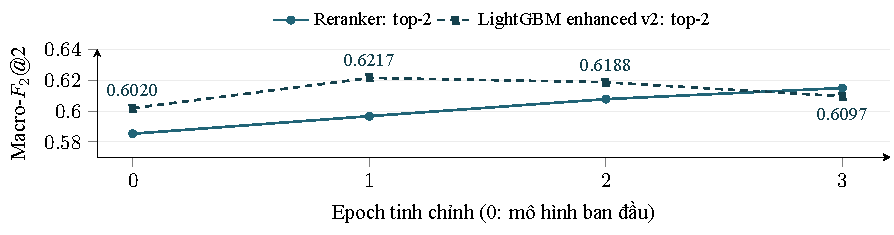
\includegraphics[width=.95\textwidth]{figures/reranker_epochs.pdf}
\caption{Macro-$F_2$@2 trước và sau LightGBM enhanced v2, cùng đầu ra top-2 trên dev.}
\label{fig:rerankerepochs}
\end{figure}


Bảng~\ref{tab:lgbm} so sánh các bộ đặc trưng từ Bảng~\ref{tab:features}, giữ reranker epoch 1, đầu ra top-2 và năm fold theo câu hỏi.
\begin{table}[H]\centering\small
\caption{So sánh các bộ đặc trưng LightGBM bằng dự đoán OOF theo câu hỏi.}\label{tab:lgbm}
\renewcommand{\arraystretch}{1.15}
\begin{tabularx}{\textwidth}{@{}Yrrrr@{}}
\toprule Mô hình / bộ đặc trưng & Số đặc trưng & P@2 & R@2 & $F_2$@2\\\midrule
Chỉ reranker & 0 & 0.4064 & 0.6759 & 0.5967\\
Cơ bản (base v1) & 15 & 0.4201 & 0.7006 & 0.6180\\
Dẫn xuất (enhanced v1) & 37 & 0.4189 & 0.6957 & 0.6145\\
\rowcolor{pale}Thống kê đoạn (enhanced v2) & 57 & \best{0.4269} & \best{0.7017} & \best{0.6217}\\
Thêm tĩnh điều luật (enhanced v3) & 65 & 0.4224 & 0.6916 & 0.6134\\\bottomrule
\end{tabularx}
\end{table}
Enhanced v2 dẫn đầu cả ba độ đo, hơn base v1 0.0037 về $F_2$@2. Bổ sung tám thống kê tĩnh ở v3 làm Recall và $F_2$ giảm; hệ thống vì vậy chọn bộ 57 đặc trưng.
% 13 — Chính sách và benchmark.
\clearpage
\subsection{Chính sách đầu ra và đối chiếu kết quả công bố}
Bảng~\ref{tab:policies} trình bày các chính sách đầu ra trên 438 câu dev với LightGBM enhanced v2. Sau khi đã chọn biểu diễn và mô hình xếp hạng, bước này khảo sát cách quyết định độ dài danh sách. Chính sách học chọn ngưỡng hoặc trọng số ở các fold trong, đánh giá ở năm fold ngoài như Phần~\ref{sec:selectors}; top-2 giữ nguyên làm đối chứng.
\begin{table}[H]\centering\small
\caption{So sánh các chính sách chọn số điều luật trên tập dev.}\label{tab:policies}
\renewcommand{\arraystretch}{1.17}
\begin{tabularx}{\textwidth}{@{}Yrrr@{}}
\toprule Chính sách & Precision & Recall & Macro-$F_2$\\\midrule
Top-2 cố định & 0.4269 & 0.7017 & 0.6217\\
Score gap & 0.5689 & 0.7076 & 0.6747\\
Fold-safe learned stopping & 0.5243 & \best{0.7303} & 0.6771\\
\rowcolor{pale}Multiclass--Ridge & \best{0.5757} & 0.7274 & \best{0.6910}\\\bottomrule
\end{tabularx}\end{table}
Chênh lệch $F_2$ giữa Multiclass--Ridge và top-2 là 0.0693. Learned stopping đạt Recall cao nhất (0.7303), còn Multiclass--Ridge giữ Recall gần mức này (0.7274) với Precision cao hơn (0.5757 so với 0.5243). Sự cân bằng đó đưa Multiclass--Ridge lên mức $F_2$ cao nhất trong các chính sách được trình bày.

Bảng~\ref{tab:benchmark} đối chiếu Macro-$F_2$ trên public và private test giữa các hệ thống tham gia DRiLL và Nhóm 18. Bản nộp của Nhóm 18 đạt 0.6978 trên public và 0.6825 trên private theo Codabench.
\begin{table}[H]\centering\small
\caption{Macro-$F_2$ toàn hệ thống trên public và private test.}\label{tab:benchmark}
\renewcommand{\arraystretch}{1.16}
\begin{tabularx}{\textwidth}{@{}Yrr@{}}
\toprule Hệ thống & Public F2 & Private F2\\\midrule
EDM & 0.5982 & \best{0.7261}\\
FPT IS & \best{0.7426} & 0.6966\\
CUDO & 0.7345 & 0.6955\\
\rowcolor{pale}\textbf{Nhóm 18} & \textbf{0.6978} & \textbf{0.6825}\\
Berry & 0.4456 & 0.6710\\
IUH.TD & 0.6337 & 0.6521\\
brain\_rot & 0.7032 & 0.6495\\
AImba & 0.6473 & 0.6425\\
Baseline two-stage (BTC) & -- & 0.5512\\
Baseline BM25 (BTC) & 0.2771 & 0.3365\\\bottomrule
\end{tabularx}\end{table}
Trên private, Nhóm 18 hơn baseline hai giai đoạn 0.1313, còn cách FPT IS 0.0141 và EDM 0.0436. Nhóm chưa làm giàu tiêu đề/tóm tắt bằng LLM như FPT IS~\cite{fpt}, hoặc bổ sung đặc trưng LLM đánh giá mức liên quan như EDM~\cite{edm}. Các thành phần này có thể giúp biểu diễn văn bản rõ hơn và phân biệt ứng viên gần nghĩa, gợi ý hướng thu hẹp khoảng cách điểm. Giả thuyết này cần được kiểm chứng bằng so sánh từng thành phần.
% 14 — Chừa chỗ phân tích lỗi, sau đó kết luận.
\clearpage
\subsection{Phân tích lỗi và trực quan hóa kết quả}
\label{sec:erroranalysis}
\begingroup
\setlength{\intextsep}{6pt}
Trên 438 câu dev có 593 cặp câu hỏi--điều luật theo gold; hệ thống trả đúng 387 cặp và bỏ sót 206 cặp. Hình~\ref{fig:errorcounts} phân các cặp bị bỏ sót thành ba nhóm không chồng lấn: không vào tập ứng viên, có trong tập nhưng ngoài top-5 sau LightGBM, hoặc nằm trong top-5 nhưng bị điểm cắt loại.
\begin{figure}[H]
\centering
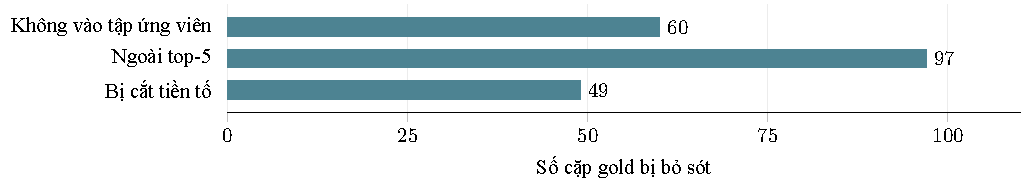
\includegraphics[width=.95\textwidth]{figures/error_counts.pdf}
\caption{Phân bố các cặp gold bị bỏ sót; top-5 xét sau LightGBM, trước chọn tiền tố.}
\label{fig:errorcounts}
\end{figure}
Các số đếm được cộng theo cặp; Recall ở Bảng~\ref{tab:policies} lấy trung bình theo câu hỏi. Nhóm ngoài top-5 chiếm nhiều nhất (97/206), gợi ý cần cải thiện thứ hạng bên cạnh chọn độ dài. Bảng~\ref{tab:errorcases} minh họa hai lỗi ở bước chọn kết quả: cắt thiếu một gold đã xếp cao và giữ thêm ứng viên cùng chủ đề nhưng ngoài nhãn.
\begin{table}[H]
\centering\small
\caption{Hai trường hợp minh họa lỗi chọn số điều luật trên tập dev.}
\label{tab:errorcases}
\renewcommand{\arraystretch}{1.12}
\begin{tabularx}{\textwidth}{@{}>{\raggedright\arraybackslash}p{4.1cm}>{\raggedright\arraybackslash}p{1.65cm}>{\raggedright\arraybackslash}p{1.65cm}Y@{}}
\toprule
Câu hỏi (qid) & Gold (aid) & Trả về (aid) & Nhận xét\\
\midrule
14663: Vi bằng phải đảm bảo nội dung và hình thức thế nào? & 29868, 29872 & 29872 & Giữ top-1 dù hai gold ở hạng 1--2 sau LightGBM; mã 29868 bị bỏ tại điểm cắt.\\
2406: Người khuyết tật được ưu tiên mua vé xe buýt không? & 19739 & 19739, 57446 & Mã 57446 nói về miễn, giảm giá vé; gần chủ đề nhưng ngoài gold của câu hỏi về ưu tiên mua vé.\\
\bottomrule
\end{tabularx}
\end{table}
\endgroup

\section{Thảo luận, kết luận và hướng phát triển}\label{sec:conclusion}
\subsection{Kết quả chính và khả năng ứng dụng}
Article window và truy xuất lai tạo tập ứng viên; reranker và LightGBM đưa bằng chứng lên đầu; Multiclass--Ridge điều chỉnh số kết quả theo câu hỏi. Cấu hình hoàn chỉnh đạt Macro-$F_2$ 0.6978 trên public và 0.6825 trên private.

Kết quả cung cấp bằng chứng cho tra cứu và RAG. Các thành phần hỏi đáp sau truy xuất chỉ phục vụ demo, nằm ngoài trọng tâm nghiên cứu.
\subsection{Hạn chế và hướng phát triển}\label{sec:limits}
Cấu hình đã được sàng lọc trên dev và chốt sau khi xem private, nên cần kiểm chứng độc lập. Giới hạn năm kết quả còn bất lợi cho câu hỏi nhiều gold. Hướng phát triển gồm làm giàu tiêu đề/tóm tắt bằng LLM như FPT IS, bổ sung đặc trưng LLM như EDM và dùng LLM lọc lại bằng chứng. Mỗi thành phần cần được đánh giá riêng, kèm chi phí xử lý.
% 15 — Tài liệu tham khảo.
\clearpage
\addcontentsline{toc}{section}{Tài liệu tham khảo}
\begingroup\small\raggedright\setlength{\parskip}{0pt}
\begin{thebibliography}{12}\setlength{\itemsep}{5pt}
\bibitem{rag} P. Lewis và cộng sự, ``Retrieval-Augmented Generation for Knowledge-Intensive NLP Tasks,'' \textit{NeurIPS}, 2020. \href{https://arxiv.org/abs/2005.11401}{arXiv:2005.11401}.
\bibitem{drill} T.-H.-Y. Vuong, T.-M. Nguyen, H.-T. Nguyen, T.-K. Dao, H.-T. Nguyen và H.-Q. Le, ``DRILL Shared Task 2025: The Challenge of Deep Retrieval in the Expansive Legal Landscape,'' \textit{VLSP}, 2025. \href{https://aclanthology.org/2025.vlsp-1.16/}{ACL Anthology: 2025.vlsp-1.16}.
\bibitem{bm25} S. Robertson và H. Zaragoza, ``The Probabilistic Relevance Framework: BM25 and Beyond,'' \textit{Foundations and Trends in Information Retrieval}, 2009. \href{https://doi.org/10.1561/1500000019}{doi:10.1561/1500000019}.
\bibitem{e5} L. Wang, N. Yang, X. Huang, L. Yang, R. Majumder và F. Wei, ``Multilingual E5 Text Embeddings: A Technical Report,'' 2024. \href{https://arxiv.org/abs/2402.05672}{arXiv:2402.05672}.
\bibitem{harrier} mainguyen9, ``VietLegal-Harrier-0.6B,'' thẻ mô hình, Hugging Face. \href{https://huggingface.co/mainguyen9/vietlegal-harrier-0.6b}{mainguyen9/vietlegal-harrier-0.6b}. Truy cập: 06/11/2026.
\bibitem{rrf} G. V. Cormack, C. L. A. Clarke và S. Buettcher, ``Reciprocal Rank Fusion Outperforms Condorcet and Individual Rank Learning Methods,'' \textit{SIGIR}, tr. 758--759, 2009. \href{https://doi.org/10.1145/1571941.1572114}{doi:10.1145/1571941.1572114}.
\bibitem{rerankbert} R. Nogueira và K. Cho, ``Passage Re-ranking with BERT,'' 2019. \href{https://arxiv.org/abs/1901.04085}{arXiv:1901.04085}.
\bibitem{vnreranker} AITeamVN, ``Vietnamese\_Reranker,'' thẻ mô hình, Hugging Face. \href{https://huggingface.co/AITeamVN/Vietnamese_Reranker}{AITeamVN/Vietnamese\_Reranker}. Truy cập: 06/11/2026.
\bibitem{lightgbm} G. Ke và cộng sự, ``LightGBM: A Highly Efficient Gradient Boosting Decision Tree,'' \textit{NeurIPS}, tập 30, 2017. \href{https://proceedings.neurips.cc/paper/2017/hash/6449f44a102fde848669bdd9eb6b76fa-Abstract.html}{Kỷ yếu NeurIPS 2017}.
\bibitem{fpt} Le Ba Hoai, Dinh Van Hung và Tran Bao Hieu, ``Data Augmentation and Hierarchical Chunking for Deep Retrieval in the Expansive Legal Landscape,'' \textit{VLSP}, tr. 127--131, 2025. \href{https://aclanthology.org/2025.vlsp-1.18/}{ACL Anthology: 2025.vlsp-1.18}.
\bibitem{edm} T. D. Pham, H. D. Nguyen và T. N. Phung, ``EDM Team's Approach in DRiLL@VLSP 2025: A Multi-Stage End-to-End Architecture for Deep Retrieval in the expansive Legal Landscape,'' \textit{VLSP}, tr. 132--139, 2025. \href{https://aclanthology.org/2025.vlsp-1.19/}{ACL Anthology: 2025.vlsp-1.19}.
\bibitem{vncorenlp} T. Vu, D. Q. Nguyen, D. Q. Nguyen, M. Dras và M. Johnson, ``VnCoreNLP: A Vietnamese Natural Language Processing Toolkit,'' \textit{NAACL: Demonstrations}, tr. 56--60, 2018. \href{https://aclanthology.org/N18-5012/}{ACL Anthology: N18-5012}.
\end{thebibliography}
\endgroup
\end{document}
